% !TEX options=--shell-escape
	\documentclass{article}
	\usepackage{amsmath,amssymb}
	\usepackage[inline]{enumitem}
	\usepackage{blindtext}
	\usepackage{booktabs}
	\usepackage{graphicx}
	\usepackage{xcolor}
	\usepackage[vmargin = 1.5in, top = 1in, bottom = 1.2in, letterpaper]{geometry}
	\usepackage{listings}
	\usepackage{courier}
	\usepackage{multicol}
	\usepackage{multirow}
	\usepackage{bm}
	\usepackage[labelformat=simple]{subcaption}
	\renewcommand\thesubfigure{(\alph{subfigure})}
	\usepackage{minted}
	\usepackage{fvextra}
	\definecolor{bg}{rgb}{0.95,0.95,0.95}
	\newminted{r}{mathescape, breaklines, linenos = true, bgcolor = bg}
	\usemintedstyle{tango}
	% \lstset{
	% basicstyle = \small\tt,
	% keywordstyle = \tt\color{blue},
	% commentstyle = \it\color[cmyk]{1,0,1,0},
	% stringstyle = \tt\color[RGB]{128,0,0},
	% %frame = single,
	% backgroundcolor = \color[RGB]{245,245,244},
	% breaklines,
	% extendedchars = false,
	% xleftmargin = 2em,
	% xrightmargin = 2em,
	% aboveskip = 1em,
	% tabsize = 4,
	% showspaces = false
	% }
	\newcommand\inner[2]{\left\langle{#1},{#2}\right\rangle}
	\DeclareMathOperator{\Corr}{Corr}
	\DeclareMathOperator{\Cov}{Cov}
	\DeclareMathOperator{\Var}{Var}
	\DeclareMathOperator{\E}{E}



	\begin{document}
	
	% \newfontfamily\courier{Courier New}

	
	\title{STAT 501 Homework 6}
	\author{Multinomial}
	\maketitle
	
	\begin{enumerate}[leftmargin = 0 em, label = \arabic*., font = \bfseries]
	\item
	\begin{enumerate}
		\item 
	We perform PCA crab dataset and calculate the proportion of variance for the first several PCs.
	\begin{rcode}
library(MASS)
crabs.data <- crabs[,-c(1,2,3)]

#1(a)
crabs.pc <- prcomp(crabs.data)



#  compute proportion of total variance explained by 
#  each component
   
   s <- crabs.pc$sdev^2                                

   pvar<-s/sum(s)
   cat("proportion of variance: ", pvar, fill=T) 

#  cumulative proportion of total variance explained 
#  by each component

   cpvar <- cumsum(s)/sum(s)
   cat("cumulative proportion of variance: ", cpvar, fill=T)
	\end{rcode}
And we get
\begin{rcode}
proportion of variance:  0.9824718 0.009055108 0.006984337 0.0009447218 0.0005440328

cumulative proportion of variance:  0.9824718 0.9915269 0.9985112 0.999456 1
\end{rcode}
We can see with first 2 PCs, 99\% of variance is explained. Then we plot the first PC scores for each observation in a scatter plot.
\begin{rcode}
   crabs.type <-as.factor(paste(crabs[,1], crabs[,2], sep = ""))
    plot(crabs.pc$x[,1],crabs.pc$x[,2],
          xlab="PC1",
          ylab="PC2",type="n")
    text(crabs.pc$x[,1],crabs.pc$x[,2],labels=crabs.type, col = rainbow(4)[as.numeric(crabs.type)])  
\end{rcode}
The plot is shown in Figure~\ref{pca}.
\begin{figure}[!htb]
	\centering
	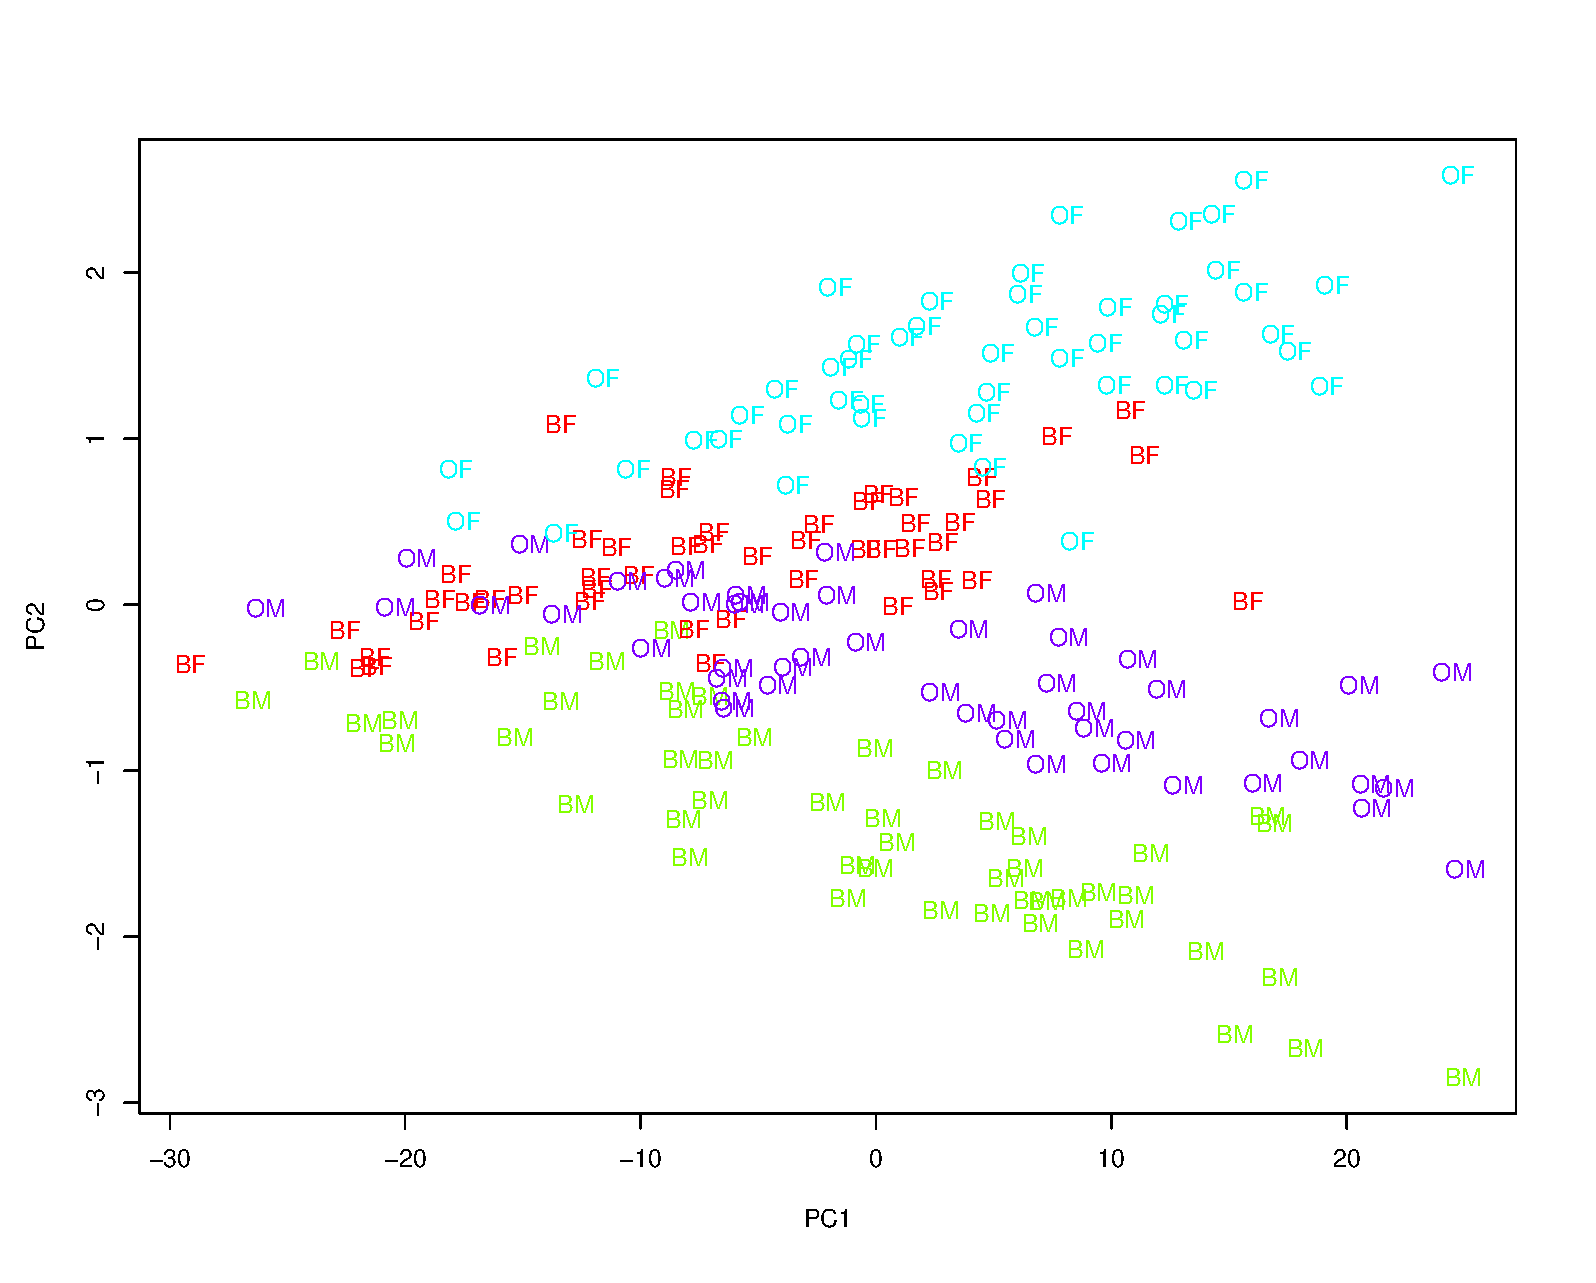
\includegraphics[width = 0.7\textwidth]{pca.eps}
	\caption{scatter plot of first two PC scores}
	\label{pca}
\end{figure}
 From the plot we can see we can kind of distiguish these 4 classes with PC1 and PC2, especially when PC1 score is large.

 We also did MANOVA with PC1 and PC2 as explanatory variables in the linear model. 
 \begin{rcode}
fit.lm <- lm(crabs.pc$x[,1:2]~as.factor(crabs.type))
library(car)
fit.manova <- Manova(fit.lm)
summary(fit.manova)
 \end{rcode}
 The result is
\begin{rcode}
Type II MANOVA Tests:

Sum of squares and products for error:
           PC1        PC2
PC1 24686.6698 -245.89146
PC2  -245.8915   50.83784

------------------------------------------
 
Term: as.factor(crabs.type) 

Sum of squares and products for the hypothesis:
          PC1      PC2
PC1 3313.7682 245.8915
PC2  245.8915 207.2327

Multivariate Tests: as.factor(crabs.type)
                 Df test stat  approx F num Df den Df     Pr(>F)    
Pillai            3  0.921355  55.80630      6    392 < 2.22e-16 ***
Wilks             3  0.165311  94.86817      6    390 < 2.22e-16 ***
Hotelling-Lawley  3  4.524930 146.30607      6    388 < 2.22e-16 ***
Roy               3  4.405940 287.85476      3    196 < 2.22e-16 ***
---
Signif. codes:  0 ‘***’ 0.001 ‘**’ 0.01 ‘*’ 0.05 ‘.’ 0.1 ‘ ’ 1
\end{rcode}
The p-value is small, so with PC1 and PC2 as explanatory variable, we can tell that these 4 classes are different.

\item 

Now we perform kernel PCA with different $\sigma = 0.2, 0.4, 0.8, 1.0, 1.5, 3.0$. We plot scatter plots for each $\sigma$ like we what did in (a).
\begin{rcode}
library(kernlab)
for(sigma in c(0.2, 0.4, 0.8, 1, 1.5, 3)){
  crabs.kpc <- kpca(x = as.matrix(crabs.data),kernel = "rbfdot", kpar = list(sigma = sigma), features = 2)
  plot(crabs.kpc@rotated[,1],crabs.kpc@rotated[,2],
       xlab="PC1",
       ylab="PC2",type="n")
  text(crabs.kpc@rotated[,1],crabs.kpc@rotated[,2],labels=crabs.type, col = rainbow(4)[as.numeric(crabs.type)])  
}
\end{rcode}  

The plots are shown in Figure~\ref{kpca}. From the plots, we can see with kernel PCA with these given $\sigma$s, we cannot distinct these 4 classes.
\begin{figure}[!htb]
    \centering
	\begin{subfigure}[b]{0.45\textwidth}
	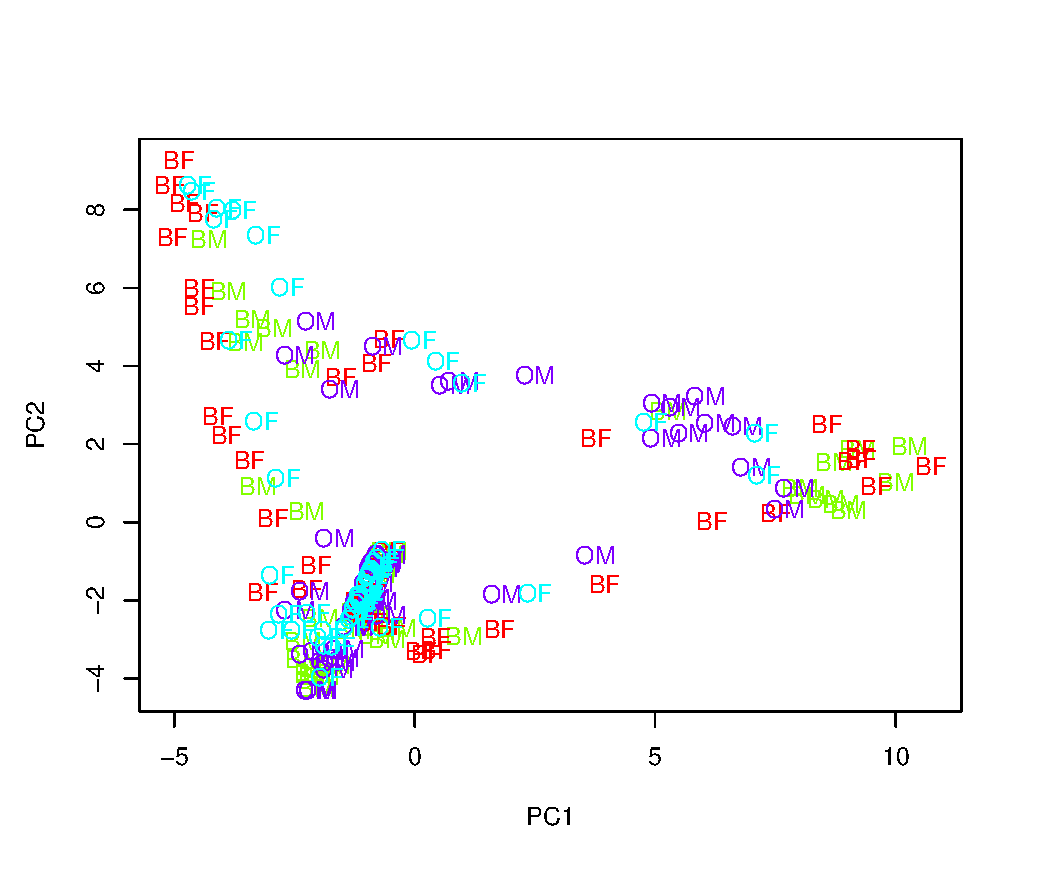
\includegraphics[width = \textwidth]{sigma02.eps}
	\caption{$\sigma = 0.2$}
	\end{subfigure}%
	\begin{subfigure}[b]{0.45\textwidth}
	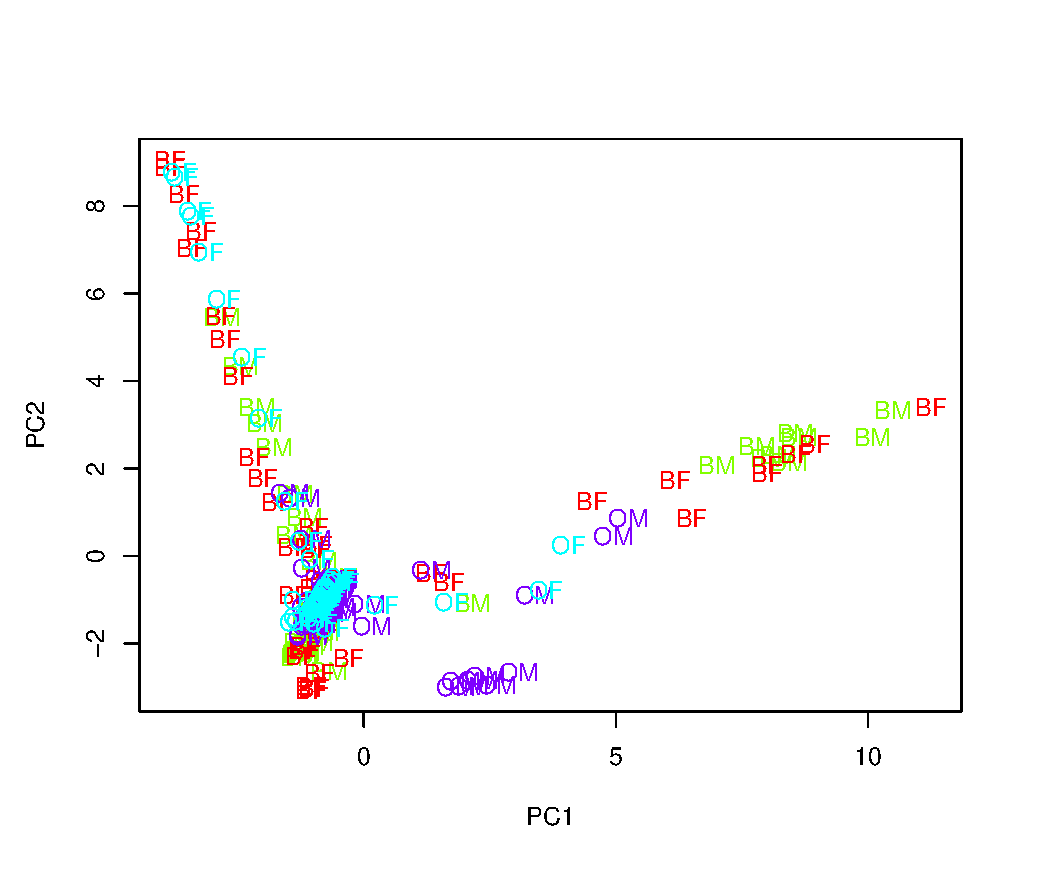
\includegraphics[width = \textwidth]{sigma04.eps}
	\caption{$\sigma = 0.4$}
	\end{subfigure}%
	\\
	\begin{subfigure}[b]{0.45\textwidth}
	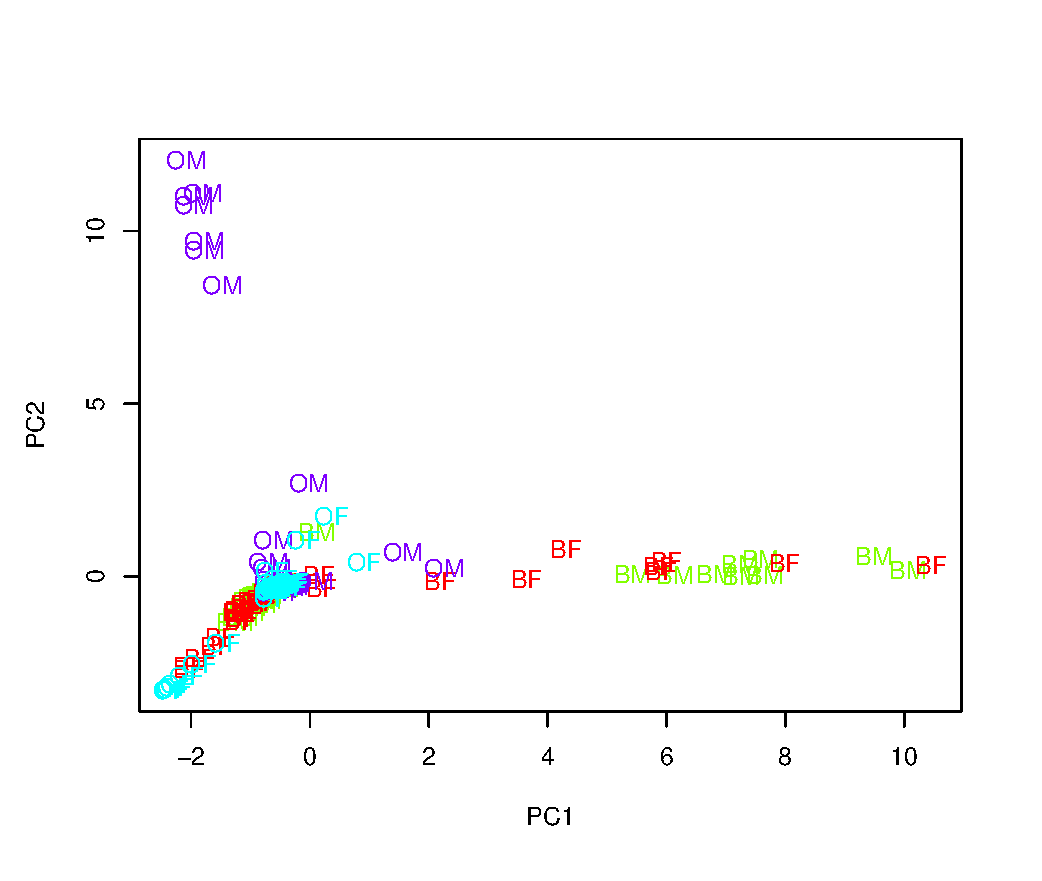
\includegraphics[width = \textwidth]{sigma08.eps}
	\caption{$\sigma = 0.8$}
	\end{subfigure}%
	\begin{subfigure}[b]{0.45\textwidth}
	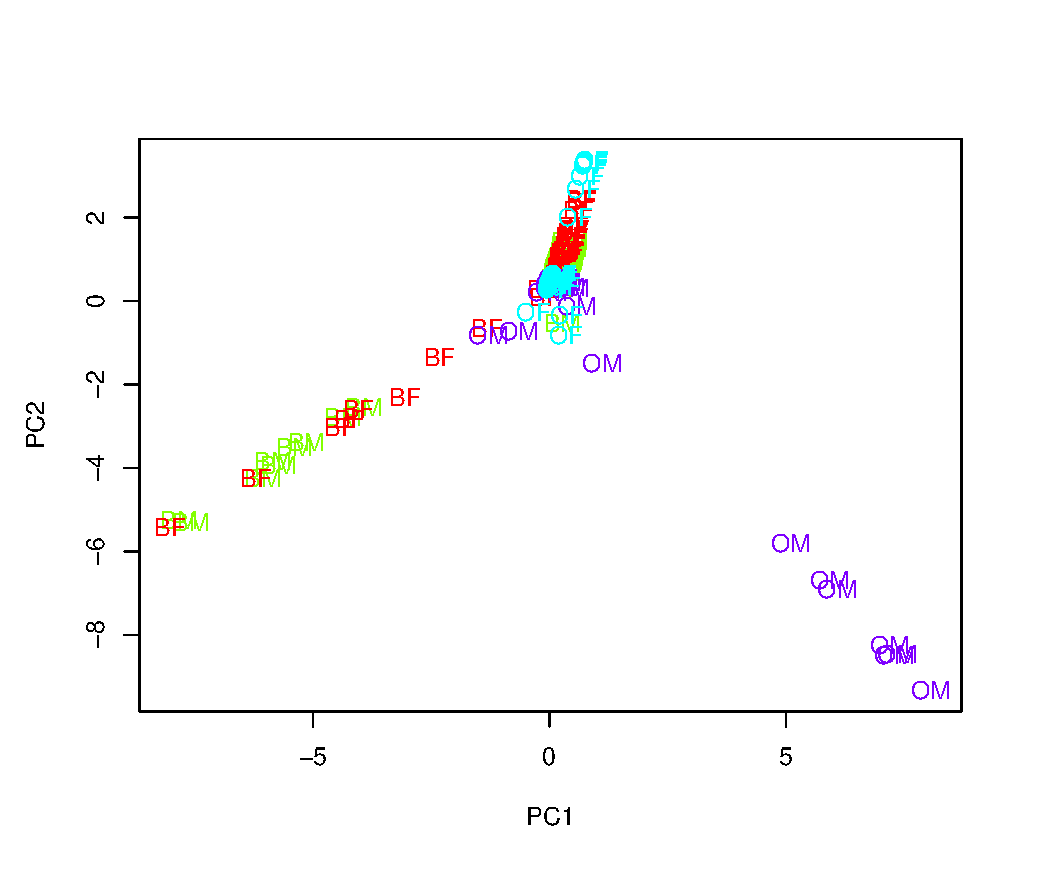
\includegraphics[width = \textwidth]{sigma1.eps}
	\caption{$\sigma = 1$}
	\end{subfigure}%
	\\
	\begin{subfigure}[b]{0.45\textwidth}
	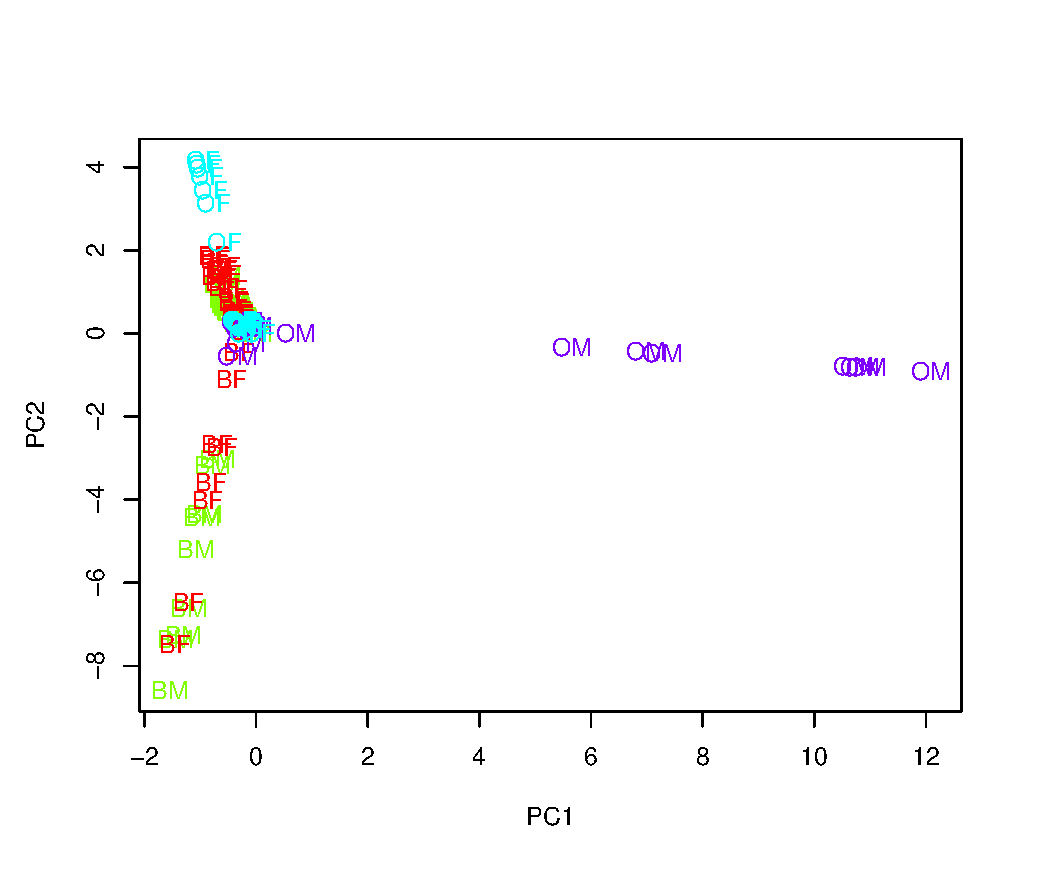
\includegraphics[width = \textwidth]{sigma15.eps}
	\caption{$\sigma = 1.5$}
	\end{subfigure}%
	\begin{subfigure}[b]{0.45\textwidth}
	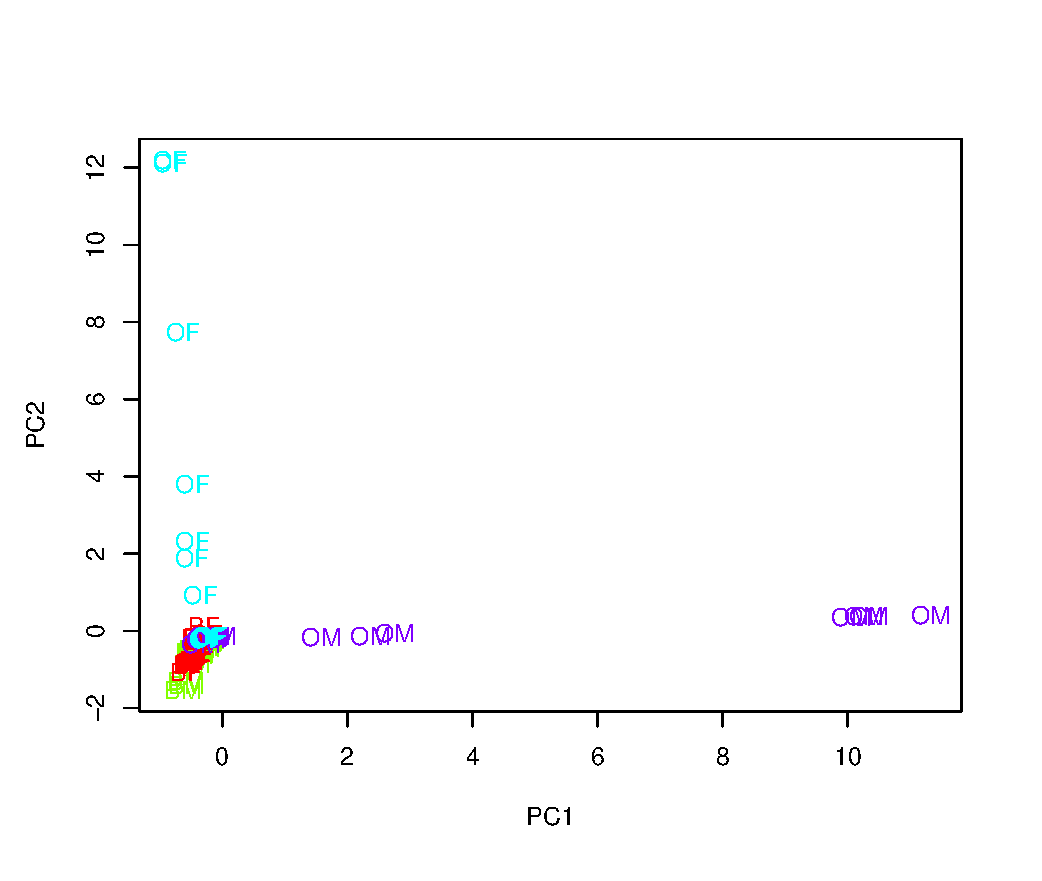
\includegraphics[width = \textwidth]{sigma3.eps}
	\caption{$\sigma = 3$}
	\end{subfigure}%
	\caption{scatter plots for scores of PC1 and PC2 from kernel PCA}
	\label{kpca}
\end{figure}
	\end{enumerate}
	\item 
	\begin{enumerate}
		\item 
		We use ANOVA to test the equality of the 10 means for each component. Then we adjust the p-values with Bonfferroni and FDR. The result shows there is only one non-significant component for Bonfferoni and no non-significant component for FDR. Then pick the 100 components with smallest p-values.
		\begin{rcode}
#2(a)
#i
ziptrain <- read.table("ziptrain.dat")
zipdigit <- as.factor(read.table("zipdigit.dat")[,1])
pval_equal_mean<- function(x, cl){
  fit <- lm(x~cl)
  return(anova(fit)[[5]][1])
}
pvals <- sapply(ziptrain, FUN = pval_equal_mean, cl = zipdigit)
pval.bonf <- p.adjust(pvals, "bonferroni")
which(pval.bonf > 0.05)
pval.fdr <- p.adjust(pvals, "fdr")
which(pval.fdr > 0.05)

id <- order(pvals, decreasing = F)
id100 <- id[1:100]

ziptrain100 <- ziptrain[,id100]

		 \end{rcode} 
		\begin{enumerate}
			\item 
			We did Box's M test to test the equality of variance covariance matrices using the data with 100 components.
			\begin{rcode}
source("BoxMTest-2.R")
BoxMTest(X = ziptrain100, cl = zipdigit)
			\end{rcode}
			The result is
			\begin{rcode}
[1] 10
------------------------------------------------
 MBox Chi-sqr. df P
------------------------------------------------
       Inf        Inf       45450       0.0000
------------------------------------------------
Covariance matrices are significantly different.
$MBox
  0 
Inf 

$ChiSq
  0 
Inf 

$df
[1] 45450

$pValue
0 
0 

			\end{rcode}
			The p-value is small and we conclude that these 10 digits' variance-covariance matrices are different.

			\item 
			Now we assume the variance-covariance matrices are not equal and they are known parameters. Let $\bm x_{ij}$ be the $j$th observation for digit $i$, $i = 0,1, \ldots, 9,\, j = 1, 2, \ldots, n_i$, then the likelihood ratio test statistic is
			\[\sum_{i=0}^{10} \sum_{j=1}^{n_i}\left[(\bm x_{ij} - \hat{\bm \mu}_{i})^T \bm \Sigma_{i}^{-1}(\bm x_{ij} - \hat{\bm \mu}) - (\bm x_{ij} - \hat{\bm \mu})^T \bm \Sigma_{i}^{-1}(\bm x_{ij} - \hat{\bm \mu}_{i})\right]\]
			where
			\begin{align*}
			& \hat{\bm \mu}_i = \sum_{j=1}^{n_i}\bm x_{ij}/n_{i}\\
			& \hat{\bm \mu} = \left(\sum_{i=0}^{\bm 10} n_{i} \bm \Sigma_{i}^{-1}\right)^{-1} \left(\sum_{i = 0}^{10} n_i \bm \Sigma_{i}^{-1} \hat{\bm \mu}_i\right)
			\end{align*}
			The R code to calculate the p-value of the likelihood ratio test is
			\begin{rcode}
			#ii
n <- as.vector(table(zipdigit))
means <- list()
for(i in 1:10){
  means[[i]] <- apply(ziptrain100[zipdigit == i-1,], MARGIN = 2, FUN = mean)
}
vars <- list()
for(i in 1:10){
  vars[[i]] <- cov(ziptrain100[zipdigit == i-1,])
}

quard <- function(x, A){
  x <- as.vector(x)
  return(t(x)%*%A%*%x)
}

lambda <- 0


r <- 0
l <- 0
for(i in 1:10){
  r <- r + n[i]*ginv(vars[[i]]) %*% means[[i]]
  l <- l + n[i]*ginv(vars[[i]])
}
muhat <- as.vector(ginv(l)%*%r)

for(i in 1:10){
  Xi <- ziptrain100[zipdigit == i-1,]
  Xicentered <- Xi - matrix(rep(means[[i]], n[i]), ncol = 100, byrow = T)
  Xim <- Xi - matrix(rep(muhat, n[i]), ncol = 100, byrow = T)
  fulli <- sum(apply(Xicentered, MARGIN = 1, FUN = quard, A = ginv(vars[[i]])))
  reducedi <-  sum(apply(Xim, MARGIN = 1, FUN = quard, A = ginv(vars[[i]])))
  lambda <- reducedi - fulli
}

pchisq(lambda, df = 9, lower.tail = F)
			\end{rcode}
			
			Then we have the test statistic \textbf{12856.64} and p-value very close to \textbf{0}. Hence we conclude that the means are different.
		\end{enumerate}
		


	\item
	\begin{enumerate}
		\item 
		We displayed the full dimension one and the reduced dimension one in Figure~\ref{pca2}. We can see the 40 dimensions one can pretty much show the variance in the full one.
		\begin{rcode}
#(b)
ziptrain.centered <- NULL
for(i in 1:10){
  mean <- apply(ziptrain[zipdigit == i-1,], MARGIN = 2, FUN = mean)
  ziptrain.centered <- rbind(ziptrain.centered, ziptrain[zipdigit == i-1,] - matrix(rep(mean, n[i]), ncol = 256, byrow = T))
}

ziptrain.pc <- prcomp(ziptrain.centered)
source("PCs.proportion.variation.enuff.R")
p <- rep(0, 256)
for(i in 1:256){
  p[i] <- PCs.proportion.variation.enuff(lambda = ziptrain.pc$sdev^2, q = i, propn = 0.8, nobs = nrow(ziptrain.centered))
}
min(which(p > 0.05))

zipmean <- NULL
for(i in 1:10){
  mean <- apply(ziptrain[zipdigit == i-1,], MARGIN = 2, FUN = mean)
  zipmean <- rbind(zipmean,  matrix(rep(mean, n[i]), ncol = 256, byrow = T))
}

zipproj_full <- ziptrain.pc$x + zipmean%*%ziptrain.pc$rotation
zipproj <- ziptrain.pc$x[,1:40] + zipmean%*%ziptrain.pc$rotation[,1:40]

source("radviz2d.R")
class <- NULL
for(i in 0:9){
  class <- c(class, rep(i, n[i+1]))
}

class <- as.factor(class)

source("starcoord.R")
starcoord(data = cbind(zipproj_full,class), class = T, main = "Full dimension")
starcoord(data = cbind(zipproj,class), class = T, main = "Reduced dimension")

		\end{rcode}

\begin{figure}[!htb]
    \centering
	\begin{subfigure}[b]{0.45\textwidth}
	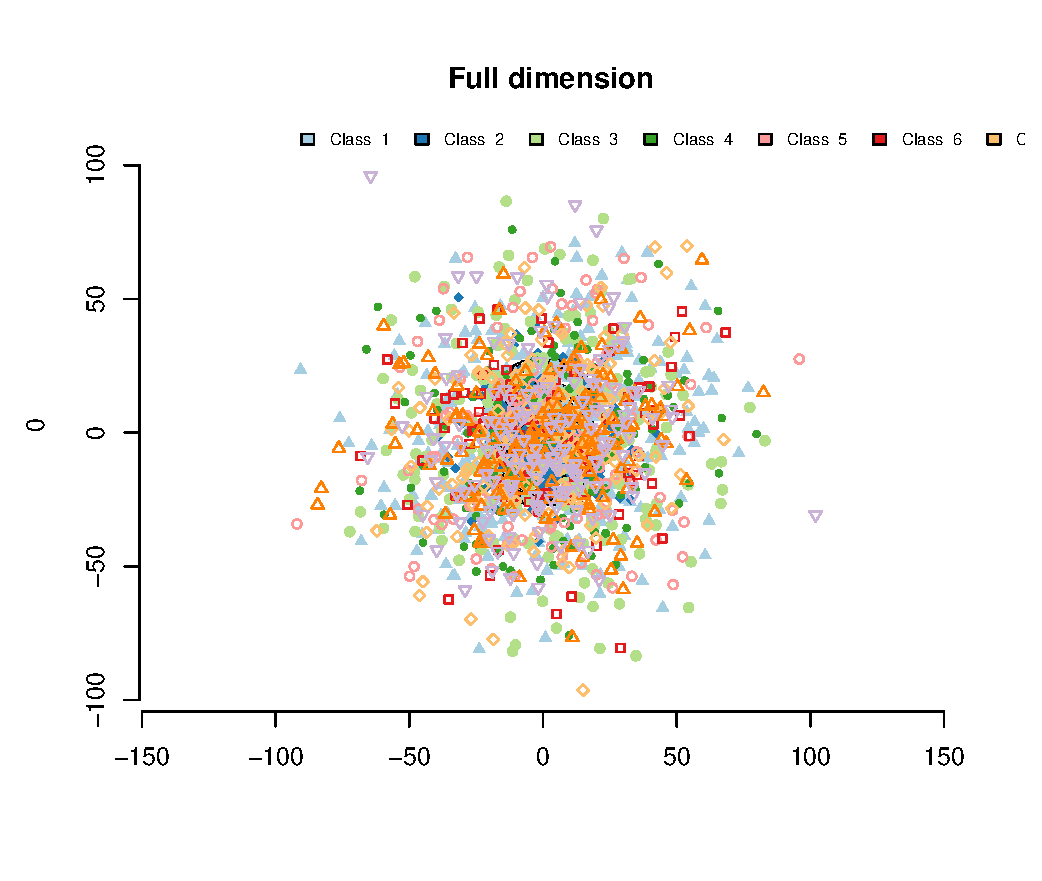
\includegraphics[width = \textwidth]{star_full.eps}
	\caption{Full dimension}
	\end{subfigure}%
	\begin{subfigure}[b]{0.45\textwidth}
	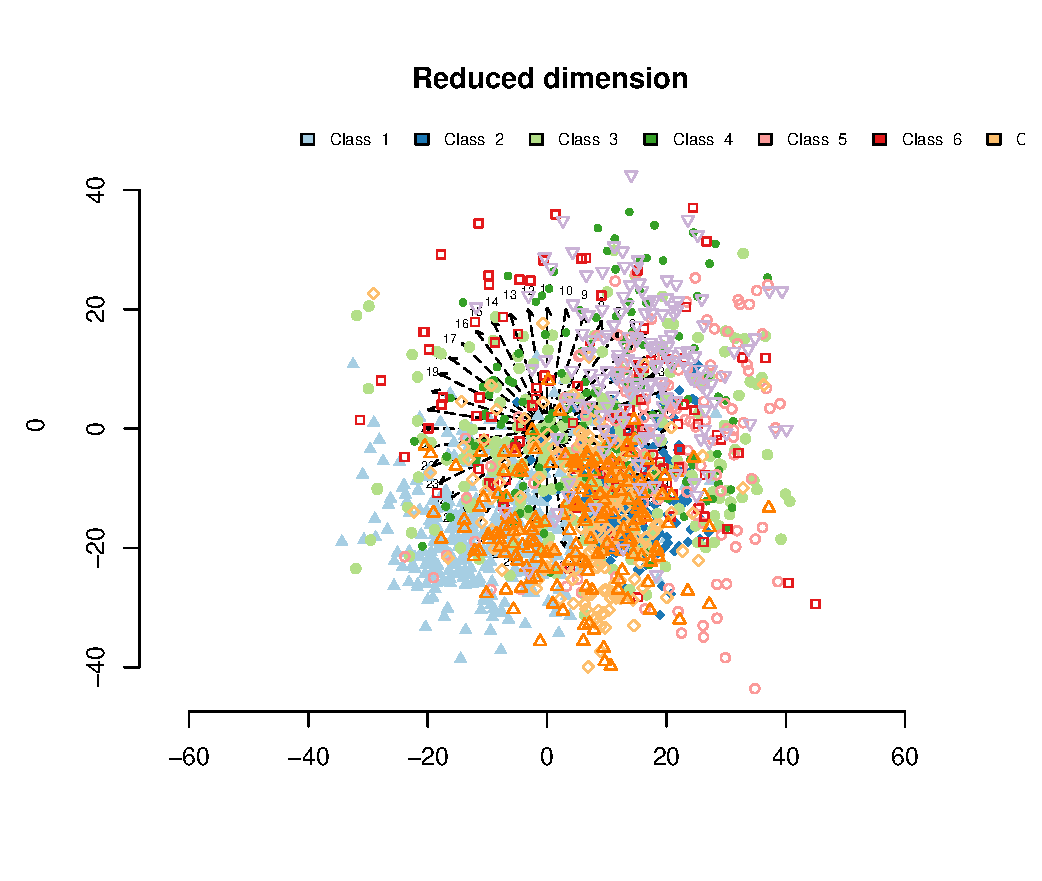
\includegraphics[width = \textwidth]{star_reduced.eps}
	\caption{Reduced dimension}
	\end{subfigure}
	\caption{Star coordinate plots}
	\label{pca2}
\end{figure}


	\end{enumerate}
	
	

	\end{enumerate}

 	\end{enumerate}









	
	
	
	\end{document}